\documentclass[12pt,a4paper]{report}
\usepackage[utf8]{inputenc}
\usepackage[english,russian]{babel}
\usepackage{indentfirst}
\usepackage{pdfpages}
\usepackage{titlesec}
\usepackage{listings}
\usepackage{amsmath}

% Вставка картинки
\usepackage{graphicx}
\graphicspath{{schemes/}}
\DeclareGraphicsExtensions{.pdf,.png,.jpg}

\usepackage[14pt]{extsizes}

\newcommand{\hsp}{\hspace{20pt}}
\titleformat{\chapter}[hang]{\large\bfseries}{\thechapter{. }}{0pt}{\large\bfseries}
\titlelabel{hlabel-formati}
\titlespacing{\chapter}{42pt}{-20pt}{12pt}
\titleformat{\section}[hang]{\large\bfseries}{\thesection{. }}{0pt}{\large\bfseries}
\titlespacing{\section}{42pt}{12pt}{5pt plus 5pt}

% Отступ абзаца
\usepackage{indentfirst}
\setlength{\parindent}{1.5cm}

% Межстрочный интервал
\usepackage{setspace}
\onehalfspacing % интервал 1.5

\usepackage[left=3cm, right=1cm, top=2cm, bottom=2cm]{geometry}

\begin{document}
% Титульник
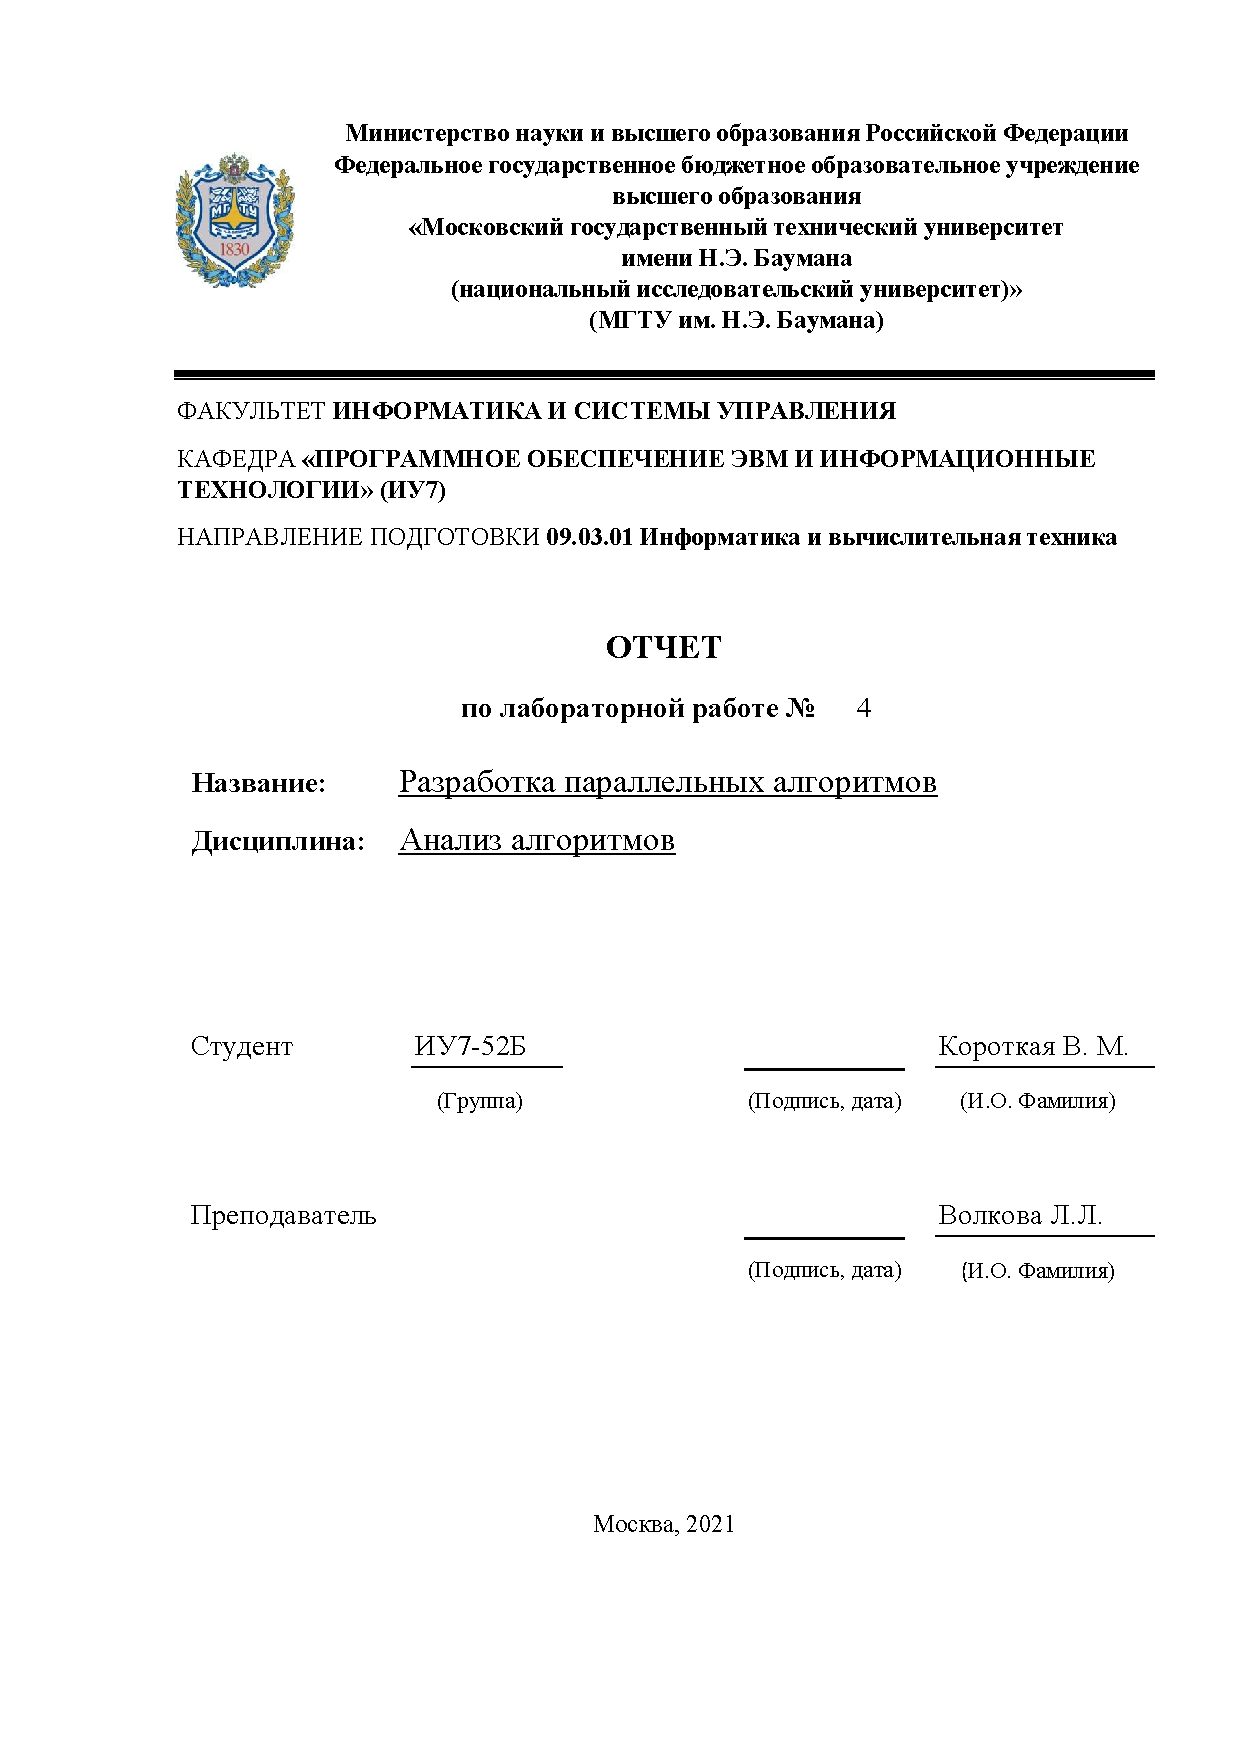
\includepdf[pages=1]{titul.pdf}
% Оглавление
\tableofcontents

\newpage
\chapter*{Введение}
\addcontentsline{toc}{chapter}{Введение}

Говоря о параллелизме в контексте компьютеров, имеется в виду,
что одна и та же система выполняет несколько независимых операций параллельно, а не последовательно.

Существует две основных причины для использования параллелизма
в приложении: 
\begin{enumerate}
    \item[-] разделение обязанностей;
    \item[-] производительность.
\end{enumerate}

Разделение обязанностей почти всегда приветствуется при разработке
программ: если сгруппировать взаимосвязанные и разделить
несвязанные части кода, то программа станет проще для понимания
и тестирования и, стало быть, будет содержать меньше ошибок.


Существует два способа применить распараллеливание для повышения производительности. 

Первый, самый очевидный, разбить
задачу на части и запустить их параллельно, уменьшив тем самым 
общее время выполнения. Это распараллеливание по задачам.  Разбиение можно формулировать как в терминах
обработки: один поток выполняет одну часть обработки, другой –
другую, так и в терминах данных: каждый поток выполняет одну и ту
же операцию, но с разными данными. Последний вариант называется
распараллеливание по данным.

Второй способ применения распараллеливания для повышения
производительности – воспользоваться имеющимся параллелизмом 
для решения более крупных задач, например, обрабатывать не один
файл за раз, а сразу два, десять или двадцать. Это по сути дела 
пример распараллеливания по данным, так как одна и та же операция 
производится над несколькими наборами данных одновременно, но
акцент немного иной. 

Целью данной работы является разработка и исследования параллельных
алгоритмов умножения матриц.

Для достижения поставленной цели необходимо выполнить следующие
задачи:

\begin{itemize}
    \item изучить основные методы параллельных вычислений,
    \item реализовать последовательный алгоритм умножения матриц,
    \item реализовать распареллелиный алгоритм умножения матриц,
    \item сравнить временные характеристики алгоритмов эксперементально.
\end{itemize}


\newpage
\chapter{Аналитическая часть}

В данном разделе будут рассмотрены алгоритм  умножения матриц и идея его параллельной реализации.

\section{Математическое описание операции умножения матриц}

Умножение матриц -- операция на матрицами $A[M * N]$ и $B[N * Q]$. 
Результатом операции является матрица C размерами M * Q, в которой каждый элемент $c_{i,j}$ задаётся 
формулой 1.1.

\begin{equation}
	c_{i,j} = \sum\limits_{k=1}^n (a_{i,k} \cdot b_{k,j})
	\label{formula:1}
\end{equation}

\section{Используемые алгоритмы}

Стандартный алгоритм подразумевает циклическое сложение всех элементов вышеописанной суммы для получения
каждого элемента матрицы C.

Параллелизм может быть достигнут за счёт выделения процессов, которые могут выполнятся независимо друг от 
друга.
В данном случае вычисление каждого элемента C ведётся независимо друг от друга, поэтому в качестве 
параллельных алгоритмов выбраны параллельное вычисление элементов строк и параллельное вычисление 
элементов столбцов.

\section*{Вывод}

Результатом аналитического раздела стало  описано понятие операции 
умножения матриц и описаны используемые алгоритмы.

Входными данными реализуемого ПО являются:

\begin{itemize}
	\item размерность первой матрицы - два натуральных числа;
	\item первая матрица - целочисленная;
	\item размерность второй матрицы - два натуральных числа;
	\item вторая матрица - целочисленная.
\end{itemize}

Выходными данными реализуемого ПО являеться результат алгоритмов умножения матриц т. е.:
\begin{itemize}
	\item матрица (результат) - для классического умножения матриц;
	\item матрица (результат) - для параллельного алгоритма умножения матриц;
	
\end{itemize}
Ограничением для реализуемого ПО является - размерность вводимых матриц т. е. длинна строки первой матрицы должна совпадать с длинной колонки второй матрицы.



\newpage
\chapter{Конструкторская часть}

В данном разделе представлены схемы алгоритмов. Так же будут описаны пользовательские структуры данных, приведены структура ПО и классы эквивалентности для тестирования реализуемого ПО.

\section{Схемы алгоритмов}

\section*{Стандартный алгоритм умножения}

Данный алгоритм непосредственно использует вышеприведённую формулу. 
Для вычисления каждого элемента матрицы C совершается циклический обход k элементов из таблиц A и B.

Схема алгоритма приведена на рисунке 2.1

\begin{figure}[ht]
	\center{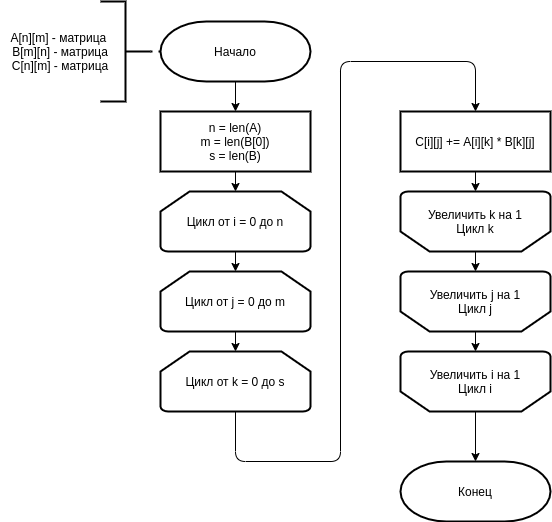
\includegraphics[scale=0.6]{classic}}
	\caption{Классический алгоритм умножения матриц.}
	%\label{fig:image}
\end{figure}'

\section*{Алгоритм умножения параллельный по строкам}

Вычисление каждого элемента матрицы является независимым. Поэтому возможна следующая параллельная 
реализация данного алгоритма. 

Пусть производится работа с T потоками. В таком случае, i-й поток будет производить вычисление строк
$i, i + T, i + 2T, \dots, ((M - i) mod T) \cdot T + i$.

Схема алгоритма приведена на рисунках 2.2 и 2.3


\begin{figure}[ht!]
	\center{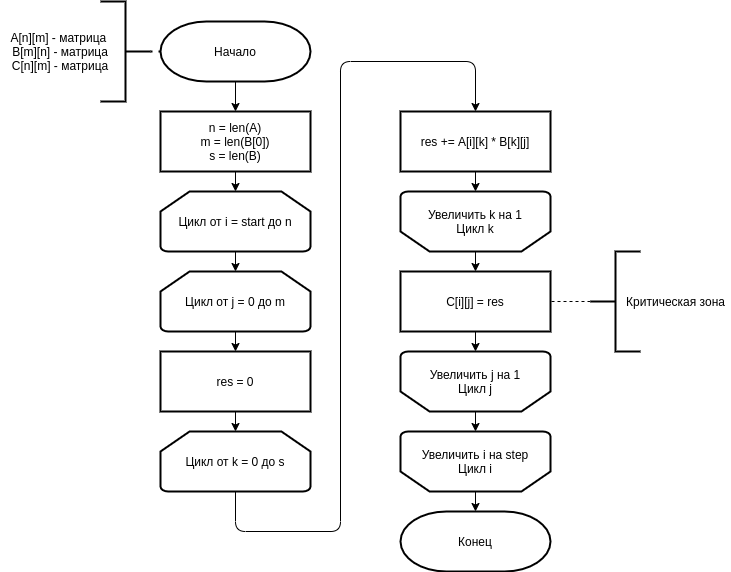
\includegraphics[scale=0.6]{parallrow1}}
	\caption{Схема параллельного умножение матриц по строкам.(часть 1)}
	%\label{fig:image}
\end{figure}


\begin{figure}[ht!]
	\center{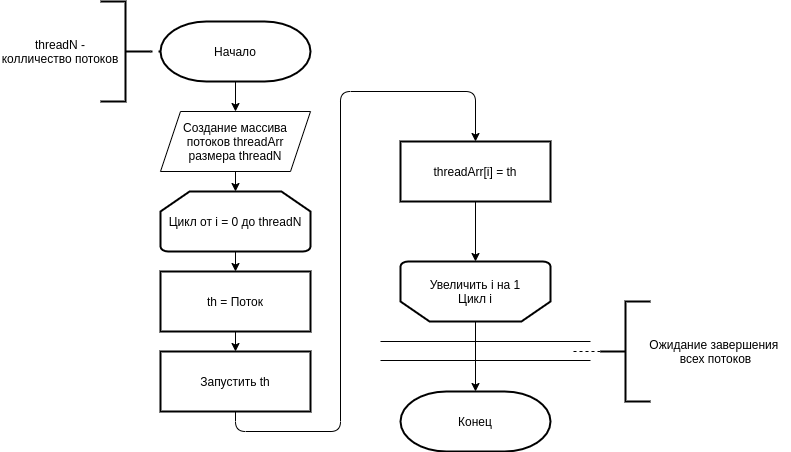
\includegraphics[scale=0.6]{parallrow2}}
	\caption{Схема параллельного умножение матриц по строкам.(часть 2)}
	%\label{fig:image}
\end{figure}


\newpage
\section{Алгоритм умножения параллельный по столбцам}

В силу независимости вычислений каждого элемента, аналогично можно организовать и параллельное вычисление
значений в столбцах матрицы C. В таком случае, i-й поток будет производить вычисление столбцов
$i, i + T, i + 2T, \dots, ((Q - i) mod T) \cdot T + i$

Схема алгоритма приведена на рисунках 2.4 и 2.5


\begin{figure}[ht!]
	\center{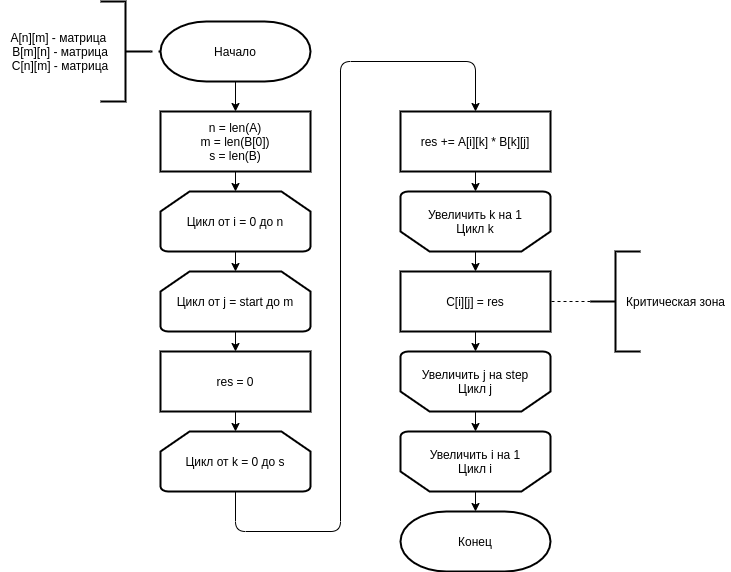
\includegraphics[scale=0.6]{parallcol1}}
	\caption{Схема параллельного умножение матриц по столбцам.(часть 1)}
	%\label{fig:image}
\end{figure}

\begin{figure}[ht!]
	\center{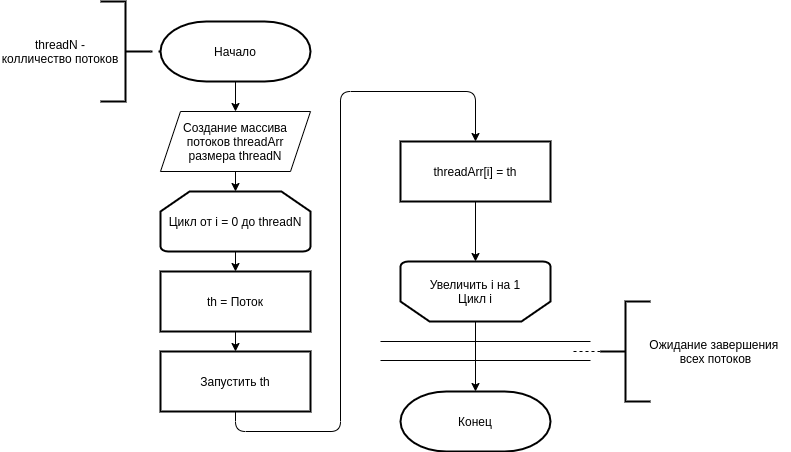
\includegraphics[scale=0.6]{parallrow2}}
	\caption{Схема параллельного умножение матриц по столбцам.(часть 2)}
	%\label{fig:image}
\end{figure}

\newpage
\section{Структура ПО}

На рисунке 2.6 представлена диограмма классов.


\begin{figure}[ht]
	\center{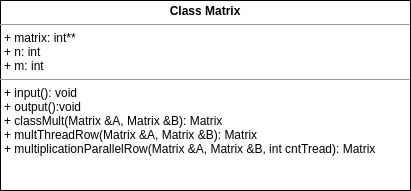
\includegraphics[scale=0.8]{structPO}}
	\caption{Диаграмма классов реализуемого ПО}
	%\label{fig:image}
\end{figure}


\section{Описание структур данных}

Для реализации данных алгоритмов, введем некоторые типы данных:

\begin{itemize}
	\item matrixType - тип данных описывающий матрицу.
\end{itemize}


\section{Тестирование}

В рамках данной лабораторной работы были выделены следующие классы эквивалентности:
\begin{itemize}
	\item входными данными являются две матрицы размерностью 1*1;
	\item входными данными являются две матрицы размерностью 1*n и n*1 соответственно;
	\item входными данными являются две матрицы квадратные матрицы равной размерностью;
	\item входными данными являются две матрицы размерностью n*k и к*т.
\end{itemize}

Для проверки работы программы будет осуществлено тестирование согласно классам эквивалентности.

\section*{Вывод}

На основе теоритических данных, полученных из аналитического раздела, были построены схемы реализируемых алгоритмов.

Так же, было приведено описание вводимых типов данных.

\newpage
\chapter{Технологическая часть} 

В данном разделе приведены средства реализации, требования к ПО и листинги кода.

\section{Средства реализации}
В качестве языка программирования был выбран с++. Данный язык знаком и предостовляет все необходимые ресурсы.
В качестве среды разработки я использовала Visual Studio Code, т.к. считаю его достаточно удобным и легким.
Visual Studio Code подходит не только для  Windows, но и для Linux, это еще одна причина, по которой я выбрала VS code, т.к. у меня установлена ОС  fedora 34.

\section{Сведенья о модулях программы}

\begin{itemize}
	\item main.cpp - файл, содержащий точку входа в программу;
	\item matrix.cpp - файл, содержащий реализацию алгоритмов умножения матриц.
\end{itemize}

\section{Реализация алгоритмов}





\noindent\textrm{Листинг 3.1: Реализация алгоритма классического умножения матриц.}
\begin{lstlisting}[frame=single, numbers=left]
matrixType classicMultiplication(matrixType a, 
                      matrixType b, int m, int n, int q)
{
    matrixType c = createMatrix(m, q);
    for (int i = 0; i < m; i++)
    {
        for (int j = 0; j < q; j++)
        {
            int res = 0;
            for (int k = 0; k < n; k++)
            {
                res += a[i][k] + b[k][j];
            }
            c[i][j] = res;
        }
    }
    return c;
}
\end{lstlisting}



\noindent\textrm{Листинг 3.2: Реализация параллельного алгоритма умножения матриц по столбцам.}
\begin{lstlisting}[frame=single, numbers=left]
void multThreadRow(matrixType& c, matrixType& a,
    matrixType&b, int m, int n, int q, int start, int step)
{
    for (int i = start; i < m; i += step)
    {
        for (int j = 0; j < q; j++)
        {
            int res = 0;
            for (int k = 0; k < n; k++)
            {
                res += a[i][k] * b[k][j];
            }
            mtx.lock();
            c[i][j] = res;
            mtx.unlock();
        }
    }
}
\end{lstlisting}


\noindent\textrm{Листинг 3.3: Реализация функции распораллеливания по столбцам.}
\begin{lstlisting}[frame=single, numbers=left]
matrixType multiplicationParallelRow(matrixType a, 
    matrixType b, int m, int n, int q, int threadCnt)
{
    matrixType c = createMatrix(m, q);
    vector<thread> threadArray;
    for (int i = 0; i < threadCnt; i++)
    {
         threadArray.push_back(thread(multThreadRow, ref(c), 
         ref(a), ref(b), m, n, q, i, threadCnt));
    }
    for (int i = 0; i < threadCnt; i++)
    {
        threadArray[i].join();
    }
    return c;
}	
\end{lstlisting}


\noindent\textrm{Листинг 3.4: Реализация параллельного алгоритма умножения матриц по строкам.}
\begin{lstlisting}[frame=single, numbers=left]
void multThreadColumn(matrixType& c, matrixType& a,
    matrixType& b, int m, int n, int q, int start, int step)
{
    for (int i = 0; i < m; i++)
    {
        for (int j = start; j < q; j += step)
        {
            int res = 0;
            for (int k = 0; k < n; k++)
            {
                res += a[i][k] * b[k][j];
            }
            mtx.lock();
            c[i][j] = res;
            mtx.unlock();
        }
    }
}
\end{lstlisting}

\noindent\textrm{Листинг 3.5: Реализация функции распораллеливания по строкам.}
\begin{lstlisting}[frame=single, numbers=left]
matrixType multiplicationParallelColumn(matrixType a,
   matrixType b, int m, int n, int q, int threadCnt)
{
    matrixType c = createMatrix(m, q);
    vector<thread> threadArray;
    for (int i = 0; i < threadCnt; i++)
    {
        threadArray.push_back(thread(multThreadColumn,
        ref(c), ref(a), ref(b), m, n, q, i, threadCnt));
    }
    for (int i = 0; i < threadCnt; i++)
    {
        threadArray[i].join();
    }
    return c;
}
\end{lstlisting}


\section{Тестирование}


В данном разделе будет приведена таблица с тестами (таблица \ref{table:ref1}).
% \ref{table:ref1}, в которой четко отражено тестирование программы

\begin{table}[ht]
	\centering
	\caption{Таблица тестов}
	\label{table:ref1}
	\begin{tabular}{ | l | l | l |}
		\hline
		Матрица A       & Матрица B           & Результат                               \\ \hline
		2 2 1 0 0 1     & 2 2 1 0 0 1         & Ответ верный                            \\ \hline
		3 2 2 3 1 0 2 2 & 2 4 2 2 1 9 4 2 8 1 & Ответ верный                            \\ \hline
		2 1 2 1         & 12 12               & Ответ верный                            \\ \hline
		2 2 1 0 0 1     & 1 1 0               & Сообщение о неверном вводе размерностей \\ \hline
		0 0             & 0 0                 &                                         \\ \hline
		\hline
	\end{tabular}
\end{table}

Все тесты пройдены.


\newpage
\chapter{Исследовательская часть} 



В данном разделе будет произведено измерение временных характеристик.

\section{Технические характеристики}


Технические характеристики устройства на котором выполнялось исследование:
\begin{itemize}
	\item процессор Intel® Core™ i5-10210U CPU @ 1.60GHz × 8;
	\item память 15.3 GiB;
	\item операционная система Fedora 34 (Workstation Edition) 64-bit.
\end{itemize}

\section{Временные характеристики}

Измерения процессорного времени проводятся на квадратных матрицах c размерами: 
32, 100, 250, 500, 1000. Содержание матриц сгенерировано случайным образом.
Изучается серия экспериментов с количеством потоков 1, 2, 3, 4, 8, 16, 32.

Для повышения точности, каждый замер производится 5 раз, за конечный результат 
берётся среднее арифметическое.

По результатам измерений процессорного времени можно составить таблицы 4.1 - 4.5.

\begin{table}[h!]
	\caption{Результаты замеров процессорного времени при размере 32 (в миллисекундах)}
	\label{tabular:timesandtenses}
	\begin{center}
		\begin{tabular}{ | l | l | l | l | l | l | l | }
			\hline
			Потоки                   & 1    & 2    & 4    & 8    & 16   & 32   \\ \hline
			Многопоточно по строкам  & 0.24 & 0.29 & 0.36 & 0.58 & 1.04 & 2.02 \\ \hline
			Многопоточно по столбцам & 0.24 & 0.30 & 0.35 & 0.59 & 1.03 & 1.97 \\ \hline
			Однопоточно              &      \multicolumn{5}{c}{0.096}   &      \\ \hline
		\end{tabular}
	\end{center}
\end{table}

\begin{table}[h!]
	\caption{Результаты замеров процессорного времени при размере 100 (в миллисекундах)}
	\label{tabular:timesandtenses}
	\begin{center}
		\begin{tabular}{ | l | l | l | l | l | l | l | }
			\hline
			Потоки                   & 1    & 2    & 4    & 8    & 16   & 32   \\ \hline
			Многопоточно по строкам  & 5.52 & 2.73 & 2.80 & 2.78 & 3.09 & 3.51 \\ \hline
			Многопоточно по столбцам & 4.87 & 3.14 & 2.87 & 2.89 & 3.15 & 3.57 \\ \hline
			Однопоточно              &      \multicolumn{5}{c}{2.96}    &      \\ \hline
		\end{tabular}
	\end{center}
\end{table}

\begin{table}[h!]
	\caption{Результаты замеров процессорного времени при размере 250 (в секундах)}
	\label{tabular:timesandtenses}
	\begin{center}
		\begin{tabular}{ | l | l | l | l | l | l | l | }
			\hline
			Потоки                   & 1     & 2     & 4     & 8     & 16    & 32    \\ \hline
			Многопоточно по строкам  & 0.068 & 0.042 & 0.031 & 0.024 & 0.026 & 0.024 \\ \hline
			Многопоточно по столбцам & 0.064 & 0.047 & 0.035 & 0.027 & 0.034 & 0.030 \\ \hline
			Однопоточно              &       \multicolumn{5}{c}{0.051}       &       \\ \hline
		\end{tabular}
	\end{center}
\end{table}

\begin{table}[h!]
	\caption{Результаты замеров процессорного времени при размере 500 (в секундах)}
	\label{tabular:timesandtenses}

\begin{center}
	\begin{tabular}{ | l | l | l | l | l | l | l | }
		\hline
		Потоки                   & 1    & 2    & 4    & 8    & 16   & 32   \\ \hline
		Многопоточно по строкам  & 0.61 & 0.38 & 0.26 & 0.20 & 0.21 & 0.20 \\ \hline
		Многопоточно по столбцам & 0.62 & 0.42 & 0.28 & 0.23 & 0.24 & 0.24 \\ \hline
		Однопоточно              &     \multicolumn{5}{c}{0.051}    &      \\ \hline
	\end{tabular}
\end{center}
\end{table}

\begin{table}[h!]
\caption{Результаты замеров процессорного времени при размере 1000 (в секундах)}
\label{tabular:timesandtenses}
\begin{center}
	\begin{tabular}{ | l | l | l | l | l | l | l | }
		\hline
		Потоки                   & 1    & 2    & 4    & 8    & 16   & 32   \\ \hline
		Многопоточно по строкам  & 8.22 & 4.63 & 2.64 & 2.18 & 2.22 & 2.27 \\ \hline
		Многопоточно по столбцам & 8.33 & 5.64 & 3.05 & 2.62 & 2.82 & 2.89 \\ \hline
		Однопоточно              &     \multicolumn{5}{c}{7.13}     &      \\ \hline
	\end{tabular}
\end{center}
\end{table}

\newpage
\section*{Вывод}

По результатам экспериментов можно заключить следующее:
\begin{itemize}
\item при относительно небольшом размере матриц (менее 100x100) использование потоков для 
уменьшения времени исполнения нецелесообразно, так как накладные расходы времени на 
управление потоками и mutex-ами больше, чем выигрыш от параллельного выполнения выполнения
вычислений;
\item использование по крайней мере двух потоков даёт ощутимый выигрыш по времени по 
сравнению с однопоточной версией алгоритма;
\item использование одного потока в многопоточных версиях алгоритма проигрывает по времени
по сравнению с однопоточной версией алгоритма, что объясняется накладными расходами времени
на управление потоками и mutex-ами;
\item использование 16 и 32 потоков показывает результат по времени несколько хуже, чем при 
8 потоках, из чего следует, что увеличение потоков даёт выигрыш по времени лишь до достижения
определённого количества, так как появляются большие накладные затраты по времени для 
управления большим количеством потоков и mutex-ов;
\item параллельные версии алгоритма выполняются за приблизительно одинаковое время при одном
потоке. Однако, использование большего количества потоков выявляет, что многопоточность по 
строкам быстрее многопоточности по столбцам вплоть до 20\%;
\item наиболее быстродейственно алгоритм действует на 8 потоках, что равно количеству 
логических процессоров на испытуемом компьютере.
\end{itemize}



%В данном разделе были приведены средства реализации, требования к ПО и листинги кода.

\newpage
\chapter*{Заключение}
\addcontentsline{toc}{chapter}{Заключение}


В данной работе были рассмотрены параллельные алгоритмы умножения матриц.

Из проведённых экспериментов было выявлено, что наиболее быстродеиственным является использование
количество потоков, которое совпадает с количеством логических процессоров процессора. 
Увеличение или уменьшение количества потоков ведёт к большему времени выполнения вычислений.
Однако, использование потоков даёт выигрыш по времени работы только для относительно больших
размеров матриц, иначе их использование лишь увеличит время вычислений за счёт накладных
расходов.
Также было установлено, что алгоритм, использующий многопоточность по строкам показывает себя
несколько быстрее алгоритма с многопоточностью по столбцам.

Цель лабороторной работы достигнутаю Выполнены поставленные задачи:

\begin{itemize}
	\item изучены основные методы параллельных вычислений,
	\item реализован последовательный алгоритм умножения матриц,
	\item реализован распареллелиный алгоритм умножения матриц,
	\item проведено сравнение временных характеристики алгоритмов эксперементально.
\end{itemize}

\newpage
\renewcommand\bibname{Список литературы}
\addcontentsline{toc}{chapter}{Список литературы}
\makeatletter % список литературы
\def\@biblabel#1{#1. }
\makeatother
\begin{thebibliography}{2}
    \bibitem{analyse_info} Дж. Макконнел. Анализ алгоритмов. Активный обучающий подход. -- М.: Техносфера, 2017. -- 267с.
    \bibitem{anatyse_info}Основы программирования на языках Си и C++ для начинающих[Электронный ресурс]. Режим доступа: http://cppstudio.com/ (дата обращения 10.10.2021)
    \bibitem{analyse_info}LINUX.ORG.RU - Русскоязычная информация о ОС Linux[Электронный ресурс] Режим доступа://www.linux.org.ru/(дата обращения 25.10.2021)
    \bibitem{analyse_info}  Документация языка C++ 98 [Электронный ресурс], режим доступа: http://www.open-std.org/JTC1/SC22/WG21/ (дата обращения 10.12.2021)
    \bibitem{analyse_info}Кнут Д. Э. Искусство программирования. Том 3. Сортировка и поиск = The Art of Computer Programming. Volume 3. Sorting and Searching / под ред. В. Т. Тертышного (гл. 5) и И. В. Красикова (гл. 6). — 2-е изд. — Москва: Вильямс, 2007. — Т. 3. — 832 с. — ISBN 5-8459-0082-1.
\end{thebibliography}

\end{document}

